\begin{figure}[t]
    \centering

    \begin{subfigure}[t]{0.32\linewidth}
        \centering
        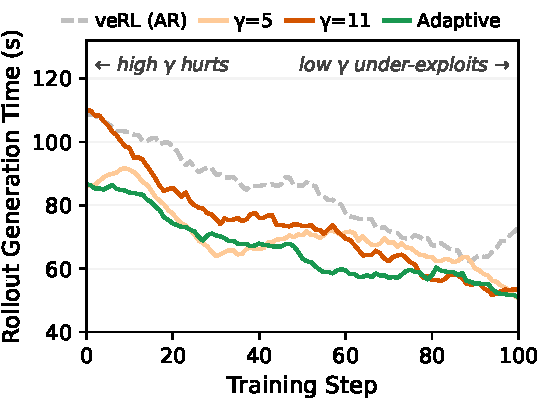
\includegraphics[width=\linewidth]{figures/main_adaptive_gen_time.pdf}
        \caption{Rollout generation time}
        \label{fig:adaptive_gamma_gen_time}
    \end{subfigure}
    \hfill
    \begin{subfigure}[t]{0.32\linewidth}
        \centering
        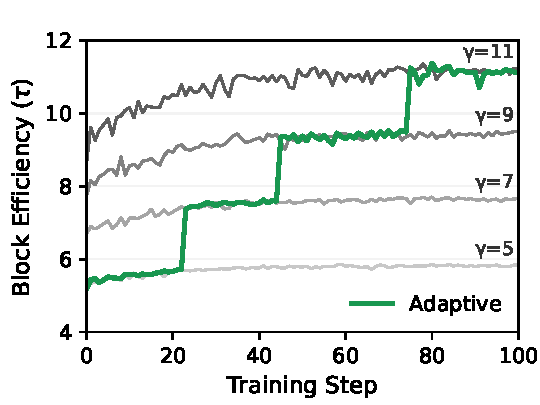
\includegraphics[width=\linewidth]{figures/main_adaptive_gamma.pdf}
        \caption{Block efficiency}
        \label{fig:adaptive_gamma_mal}
    \end{subfigure}
    \hfill
    \begin{subfigure}[t]{0.32\linewidth}
        \centering
        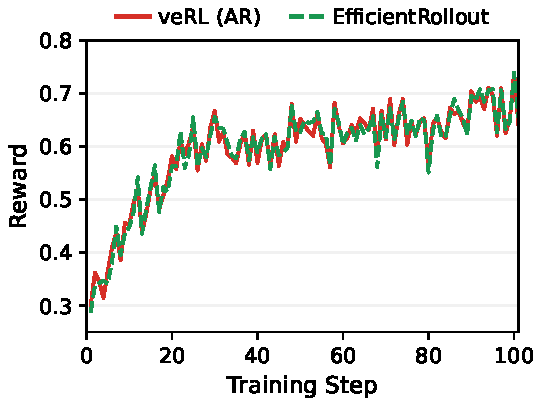
\includegraphics[width=\linewidth]{figures/appendix_fidelity_reward_qwen7b.pdf}
        \caption{Training reward}
        \label{fig:adaptive_gamma_reward}
    \end{subfigure}

    \caption{
    \textbf{Adaptive draft-length policy and training dynamics on Qwen2.5-7B.}
    (a) Adaptive $\gamma$ reduces rollout-generation time by avoiding overly large drafts early and exploiting longer drafts later.
    (b) The controller raises $\gamma$ as block efficiency $\tau$ improves during training.
    (c) \methodtitle{} follows the \nosd{} reward trajectory, indicating preserved training dynamics.
    }
    \label{fig:adaptive_gamma}
\end{figure}